\subsection{ Apparato }

Sistema ottico

I raggi paralleli all'asse ottico prodotti da una sorgente Laser vengono focalizzati in un punto $s$ da una prima lente convergente $L_{1}$.

Prima della seconda lente $L_{2}$ uno specchio semiriflettente convoglia una parte del segnale ottico ad un microscopio, utilizzato per la lettura della misura.

La seconda lente $L_{2}$, avente una distanza focale molto maggiore della prima lente $L_{1}$ ma comunque inferiore alla distanza che la separa dal punto $s$, focalizza i raggi ad una distanza $ p>f2>f1 $.

Indicativamente, con riferimento allo schema sottostante, posto $ q = f_{2}(1+\epsilon) $, la distanza tra il punto $s$ e la lente $L_{2}$ si ha che
$ \epsilon = 0.19 $ e $ p = 6 f_{2} $.

    \begin{figure}[H]
    \centering
    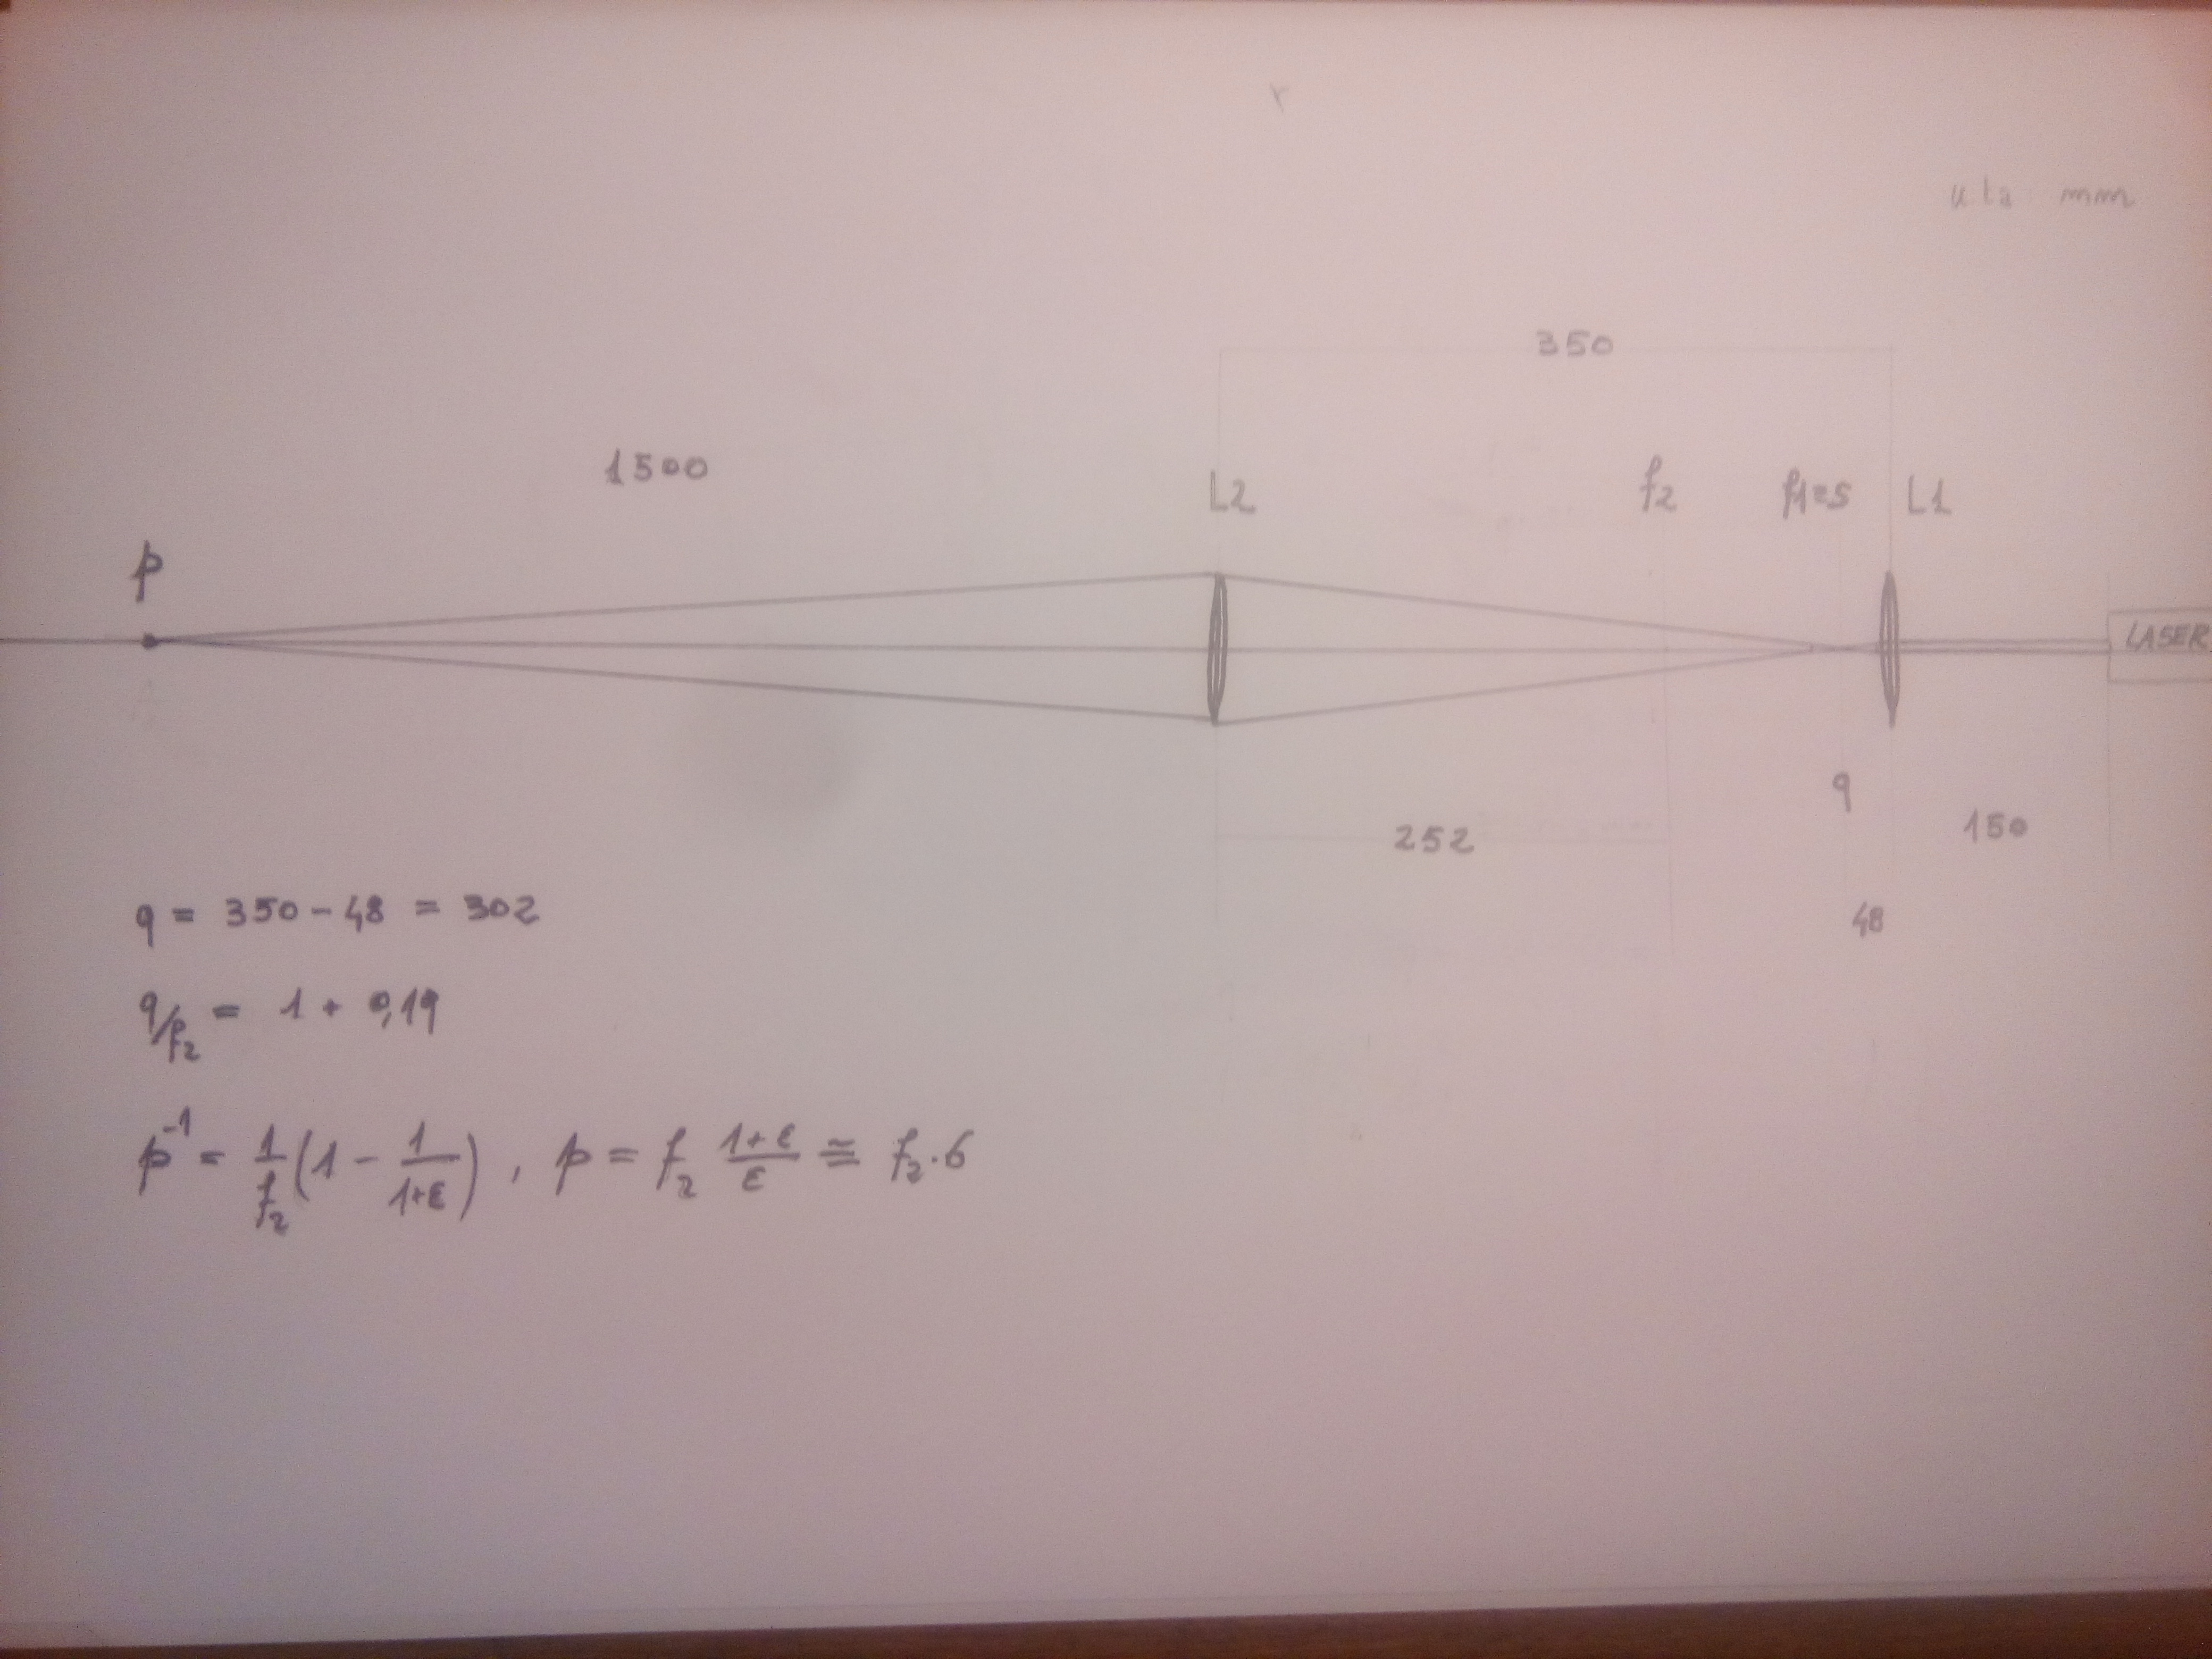
\includegraphics[scale=0.05]{Grafici/O1_P0_tavola1.jpg}
    %\caption{}
    \label{fig:C3_P2_RL}
    \end{figure} 

Prima del punto $A$ si trova interposto uno specchio imperniato su un supporto rotante che direziona i raggi verso uno specchio sferico di raggio $\sim A$; ciò fa sì che i raggi riflessi dallo specchio sferico ritornino sempre allo specchio rotante.



\subsection{ Propagazione errori }

Dalla formula che restituisce la velocità della luce
\begin{equation}
 c = 8\pi\frac{B+D}{B+D-f}fD^{2}\frac{w_{dx} + w_{sx}}{(D+B)\Delta} \quad,
\end{equation}
usando la stessa velocità in entrambi i sensi $ w_{dx} = w_{sx} = w $,
e trascurando la costante moltiplicativa $ 16\pi $, si ottiene
\begin{equation}
 c \propto \frac{fD^{2}}{B+D-f}\frac{ w }{ \Delta } \quad.
\end{equation}
L'errore relativo del primo fattore $ R = \tfrac{fD^{2}}{B+D-f} $
si stima con le formule di propagazione e con l'approssimazione
$ D+B-f \sim D  $, siccome $ D = 4980 $, e $ f = 252 $, $ B=310 $,
\begin{align*}
 \partial_{D} R & = ( D+B-f )^{-2}Df( 2(D+B-f) - D ) \sim f		\\
 \partial_{f} R & = ( D+B-f )^{-2}Df( 2(D+B-f) + D ) \sim 3f	
\end{align*}
Da cui, l'errore relativo
\begin{equation}
\epsilon_{R} = \frac{f}{R} \sqrt( 9\sigma_{f}^{2} + \sigma_{D}^{2} )
\end{equation}

%%%%%%%%%%%%%%%%%%%%%%
%%% TABELLA: calcolo errore relativo del primo fattore R

\begin{table}[htbp]
\begin{center}
\begin{tabular}{|c|c|c|c|c|c|c|}
\hline
$f$ & $D$ & $B$ & $R$ & $\sigma_{f}^{2}$ & $\sigma_{D}^{2}$ & $\epsilon_{R}$ \\ \hline
$mm$ & $mm$ & $mm$ & $mm$ & $mm^2$ & $mm^2$ &   \\ \hline
\multicolumn{1}{|r|}{$  252\pm 2 $} & \multicolumn{1}{r|} {$ 4980\pm 5 $} & \multicolumn{1}{r|} {$  310\pm 2 $} & \multicolumn{1}{r|} {$ 1.32 10^6 $} & \multicolumn{1}{r|}{4} & \multicolumn{1}{r|}{25} & \multicolumn{1}{r|} {$ 0.149\% $} \\ \hline
\end{tabular}
\end{center}
\caption{ $\sigma$ errore assoluto. $ \epsilon $ errore relativo.}
\label{=O1_P0}
\end{table}


\paragraph{Conclusioni}

Il micrometro posto sul telescopio permette di leggere misure dell'ordine del centesimo di millimetro. Tenuto conto anche della larghezza dello spot, l'errore assoluto commesso sullo spostamento non può essere inferiore a $ \pm 0.1 $ $mm$, o $ \pm 1 \% $  in termini relativi, su spostamenti dell'ordine di circa $10$ $mm$.

Trattandosi, nel caso della misura con micrometro, di misure ripetibili, trovano spazio i benefici del campionamento ripetuto, con un fattore di abbattimento proporzionale alla radice dell'ampiezza campionaria.

\begin{table}[htbp]
\begin{center}
\begin{tabular}{|c|c|c|c|c|c|}
\hline
$n$ & 10 & 20 & 30 & 40 & 50 \\ \hline
$\sqrt(n)$ & 3.16 & 4.47 & 5.48 & 6.32 & 7.07 \\ \hline
\end{tabular}
\end{center}
\caption{Fattore di abbattimento per campionamento ripetuto sulla media aritmetica dello spostamento}
\label{=O1_P0_1}
\end{table}

Affinchè l'errore sullo spostamento dello spot $ \Delta $ sia confrontabile nell'ordine di grandezza con gli altri due fattori che incidono sulla misura di $ c $, posto trascurabile l'errore sulla frequenza di rotazione dello specchio rotante, l'ampiezza campionaria desiderabile è dell'ordine delle decine.



\subsection{ Misure }

\begin{table}[htbp]
\begin{center}
\begin{tabular}{|c|c|c|c|c|c|c|c|c|c|c|c|}
\hline
$n$ & $w$ & $Pa$ & $Pb$ & \multicolumn{2}{c|}{$c$}  &  & $w$ & $Pa$ & $Pb$ & \multicolumn{2}{c|}{$c$}  \\ \hline
 & $Hz$ & $mm$ & $mm$ & \multicolumn{2}{c|}{$m/s$}  &  & $Hz$ & $mm$ & $mm$ & \multicolumn{2}{c|}{$m/s$}  \\ \hline
 &  & \multicolumn{1}{r|}{0.05} & \multicolumn{1}{r|}{0.05} & \multicolumn{2}{c|}{1.00$\%$}  &  &  & \multicolumn{1}{r|}{0.05} & \multicolumn{1}{r|}{0.05} & \multicolumn{2}{c|}{1.00$\%$}   \\ \hline
\multicolumn{1}{|r|}{1} & \multicolumn{1}{r|}{1500} & \multicolumn{1}{r|}{12.77} & \multicolumn{1}{r|}{13.07} & \multicolumn{1}{r|}{311774738} &  &  & \multicolumn{1}{r|}{750} & \multicolumn{1}{r|}{12.49} & \multicolumn{1}{r|}{12.68} & \multicolumn{1}{r|}{245893912} &  \\ \hline
 &  &  &  &  & \multicolumn{1}{r|}{292288817} &  &  &  &  &  & \multicolumn{1}{r|}{311774738} \\ \hline
\multicolumn{1}{|r|}{2} & \multicolumn{1}{r|}{1500} & \multicolumn{1}{r|}{12.75} & \multicolumn{1}{r|}{13.07} & \multicolumn{1}{r|}{292288817} &  &  & \multicolumn{1}{r|}{750} & \multicolumn{1}{r|}{12.53} & \multicolumn{1}{r|}{12.68} & \multicolumn{1}{r|}{311465622} &  \\ \hline
 &  &  &  &  & \multicolumn{1}{r|}{301717488} &  &  &  &  &  & \multicolumn{1}{r|}{359740082} \\ \hline
\multicolumn{1}{|r|}{3} & \multicolumn{1}{r|}{1500} & \multicolumn{1}{r|}{12.76} & \multicolumn{1}{r|}{13.05} & \multicolumn{1}{r|}{322525591} &  &  & \multicolumn{1}{r|}{750} & \multicolumn{1}{r|}{12.55} & \multicolumn{1}{r|}{12.69} & \multicolumn{1}{r|}{333713166} &  \\ \hline
 &  &  &  &  & \multicolumn{1}{r|}{359740082} &  &  &  &  &  & \multicolumn{1}{r|}{233831053} \\ \hline
\multicolumn{1}{|r|}{4} & \multicolumn{1}{r|}{1500} & \multicolumn{1}{r|}{12.79} & \multicolumn{1}{r|}{13.09} & \multicolumn{1}{r|}{311774738} &  &  & \multicolumn{1}{r|}{750} & \multicolumn{1}{r|}{12.49} & \multicolumn{1}{r|}{12.68} & \multicolumn{1}{r|}{245893912} &  \\ \hline
 &  &  &  &  & \multicolumn{1}{r|}{283431580} &  &  &  &  &  & \multicolumn{1}{r|}{259812282} \\ \hline
\multicolumn{1}{|r|}{5} & \multicolumn{1}{r|}{1500} & \multicolumn{1}{r|}{12.76} & \multicolumn{1}{r|}{13.07} & \multicolumn{1}{r|}{301717488} &  &  & \multicolumn{1}{r|}{750} & \multicolumn{1}{r|}{12.5} & \multicolumn{1}{r|}{12.69} & \multicolumn{1}{r|}{245893912} &  \\ \hline
 &  &  &  &  & \multicolumn{1}{r|}{311774738} &  &  &  &  &  & \multicolumn{1}{r|}{246137951} \\ \hline
\multicolumn{1}{|r|}{6} & \multicolumn{1}{r|}{1500} & \multicolumn{1}{r|}{12.77} & \multicolumn{1}{r|}{13.08} & \multicolumn{1}{r|}{301717488} &  &  & \multicolumn{1}{r|}{750} & \multicolumn{1}{r|}{12.5} & \multicolumn{1}{r|}{12.68} & \multicolumn{1}{r|}{259554685} &  \\ \hline
 &  &  &  &  & \multicolumn{1}{r|}{334044362} &  &  &  &  &  & \multicolumn{1}{r|}{246137951} \\ \hline
\multicolumn{1}{|r|}{7} & \multicolumn{1}{r|}{1500} & \multicolumn{1}{r|}{12.8} & \multicolumn{1}{r|}{13.08} & \multicolumn{1}{r|}{334044362} &  &  & \multicolumn{1}{r|}{750} & \multicolumn{1}{r|}{12.49} & \multicolumn{1}{r|}{12.67} & \multicolumn{1}{r|}{259554685} &  \\ \hline
 &  &  &  &  & \multicolumn{1}{r|}{292288817} &  &  &  &  &  & \multicolumn{1}{r|}{275095357} \\ \hline
\multicolumn{1}{|r|}{8} & \multicolumn{1}{r|}{1500} & \multicolumn{1}{r|}{12.76} & \multicolumn{1}{r|}{13.07} & \multicolumn{1}{r|}{301717488} &  &  & \multicolumn{1}{r|}{750} & \multicolumn{1}{r|}{12.5} & \multicolumn{1}{r|}{12.68} & \multicolumn{1}{r|}{259554685} &  \\ \hline
 &  &  &  &  & \multicolumn{1}{r|}{301717488} &  &  &  &  &  & \multicolumn{1}{r|}{246137951} \\ \hline
\multicolumn{1}{|r|}{9} & \multicolumn{1}{r|}{1500} & \multicolumn{1}{r|}{12.76} & \multicolumn{1}{r|}{13.09} & \multicolumn{1}{r|}{283431580} &  &  & \multicolumn{1}{r|}{750} & \multicolumn{1}{r|}{12.49} & \multicolumn{1}{r|}{12.68} & \multicolumn{1}{r|}{245893912} &  \\ \hline
 &  &  &  &  & \multicolumn{1}{r|}{292288817} &  &  &  &  &  & \multicolumn{1}{r|}{311774738} \\ \hline
\multicolumn{1}{|r|}{10} & \multicolumn{1}{r|}{1500} & \multicolumn{1}{r|}{12.77} & \multicolumn{1}{r|}{13.08} & \multicolumn{1}{r|}{301717488} &  &  & \multicolumn{1}{r|}{750} & \multicolumn{1}{r|}{12.83} & \multicolumn{1}{r|}{12.98} & \multicolumn{1}{r|}{311465622} &  \\ \hline
\end{tabular}
\end{center}
\caption{Tabella a sinistra $ w=1500 $ $Hz$. Tabella a destra $ w=750 $ $Hz$. Velocità della luce $c$ $[m/s]$: la prima colonna relativa a $c$ riporta la stima relativa allo spostamento $Pb_{i}-Pa_{i}$. La seconda è relativa a $ Pb_{i-1} - Pa_{i} $.}
\label{O1_P2}
\end{table}


%
% Istogrammi
%
    \begin{figure}[H]
    \centering
    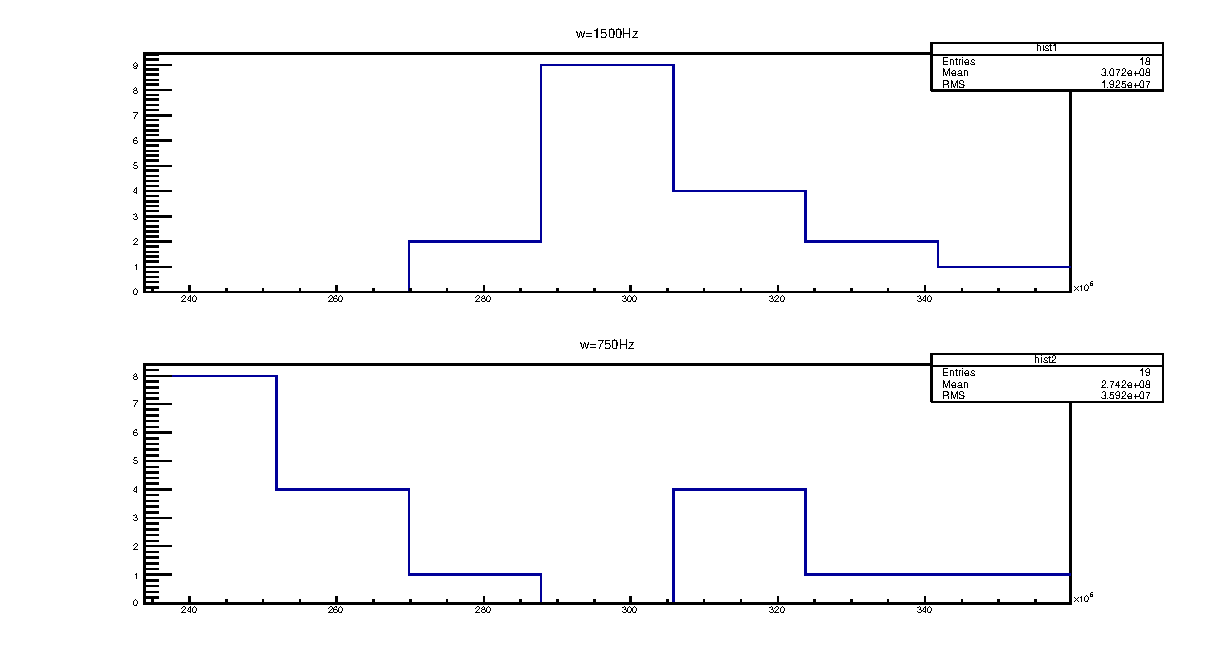
\includegraphics[scale=0.8]{Grafici/O1_P2_c.eps}
    \caption{Istogramma misure di $c$ [m/s].}
    \label{fig:O1_P2_c}
    \end{figure} 
%